%-------------------------------------------------------------------------------
\section{Introduction}
%-------------------------------------------------------------------------------    

The relationship between Internet transport protocols and lossy
wireless networks has long been fraught. Three decades ago, the
seminal Snoop work~\cite{balakrishnan1995snoop} addressed an issue
that emerged with the rise of wireless Ethernet (Wi-Fi): TCP's
end-to-end reliability works poorly over network segments that
regularly experience non-congestive packet loss. This is for two big
reasons: it's wasteful to require frequent end-to-end retransmissions
over a whole network path to address packet loss on one wireless link,
and because most congestion-control schemes interpret packet loss as a
sign of congestion and will slow down in response---a mistake when the
loss wasn't caused by congestion. From its point of view in 1995, the
Snoop paper outlined three plausible solutions:
\begin{itemize}[topsep=0pt,itemsep=0pt]
\item \textbf{Splitting TCP connections}~\cite{bakreitcp1994, bb95}. A
  proxy at the wireless base station transparently interposes on TCP
  connections that cross it, creating two concatenated connections:
  one from ``fixed host'' to proxy, and from proxy to the ``mobile
  host.'' This lets retransmission occur over the lossy segment only,
  and prevents the fixed host's congestion control from seeing
  non-congestive wireless losses.

\item \textbf{Link-level acknowledgment and
  retransmission}~\cite{palplus}. Wireless NICs add their own
  encapsulation (with their own sequence numbers or packet
  identifiers) to each packet, reply to incoming packets with
  link-layer acknowledgments, detect apparent losses from the absence
  of an ACK, and retransmit lost packets before the end-to-end
  transport protocol concludes they were lost.

\item \textbf{The Snoop approach}, where an on-path network function
  transparently interprets TCP acknowledgments in-flight, detects
  losses, retransmits packets over the lossy link only, and
  temporarily hides loss from the other host to avoid a duplicate
  retransmission.
\end{itemize}

In the intervening years, the first two approaches were widely
deployed. At the boundary between the wired Internet and a lossy
wide-area subpath (e.g.~a satellite or cellular network), network
operators used connection-splitting performance-enhancing proxies
(PEPs) to accelerate TCP connections crossing their networks. For
lossy \emph{local}-area subpaths, Wi-Fi and cellular networks use
link-layer sequence numbers, selective ``block'' acknowledgments,
link-layer retransmissions, and receiving NICs that sometimes hold
back received packets to wait for retransmissions of earlier packets
so that hosts receive packets in the original order to avoid
triggering a transport-layer end-to-end retransmission~\cite{rfc3366,
  rfc8985, 802.1ac, 5Greorder}. Because of the practical success of
the first two approaches, Snoop's ``network-originated
retransmissions'' didn't seem to be needed in practice.

Until, this paper proposes, maybe now. Post-TCP transport protocols,
especially QUIC~\cite{rfc9000}, encrypt and authenticate their
packets. This puts some operators in a bind, because they can no longer
``split'' these connections.
But what about link-layer ACKs and retransmissions?
This is a usable strategy on low-latency wireless links when one party
(or standards body) controls both sides, and losses can be patched
before the end-to-end protocol detects them. But when the lossy
subpath has higher latency (as for some satellite or experimental
networks), losses can't be patched before the transport protocol
detects them, and the head-of-line blocking necessary to put
packets back in order at the receiver can be ruinous to real-time
applications. In any event, such techniques can't be deployed
unilaterally by a network operator who doesn't control the receiver or
the encapsulation format.

What else could address this? Traffic sources could deploy
congestion-control and loss-detection schemes that are less sensitive
to loss and reordering~\cite{rfc8985}, but this is also out of a
network operator's control. Yet another approach could involve
Sidekick proxies~\cite{yuan2024sidekick}---but these provide
in-network \emph{acknowledgments} of encrypted transport protocols
(for hosts to interpret and perhaps trigger retransmission), not
in-network \emph{retransmission} based on the encrypted traffic of
hosts.

Given all this, what really happens today, at least some
of the time, is that satellite and other nontraditional network
operators block QUIC traffic, forcing hosts to fall back to TCP that
can be split as before. We think it may be possible to do better by drawing on ``Snoop-style''
ideas. In this paper, we describe and evaluate \Sys\footnote{For
``packet rateless retransmission''---and because the \Sys proxy keeps
a small cache of recent packets-in-flight for possible
retransmission.}: a technique for network-originated retransmissions
for encrypted end-to-end transport connections, yielding performance
benefits in lossy settings. We adapt set-reconciliation techniques
based on the Rateless IBLT~\cite{yang2024practical} to let the
receiver efficiently acknowledge encrypted packets (in an ``eACK'') to a network
function, without modifying the sender or the underlying wire
format. Compared with Sidekick, which also involves
acknowledgments over encrypted sequence numbers, these eACKs
are faster to decode, making them appropriate for a deployment
where network functions are the ones interpreting acknowledgments over
encrypted sequence numbers from many connections in parallel and
triggering retransmissions as a result.

% \begin{figure}
%     \centering
%     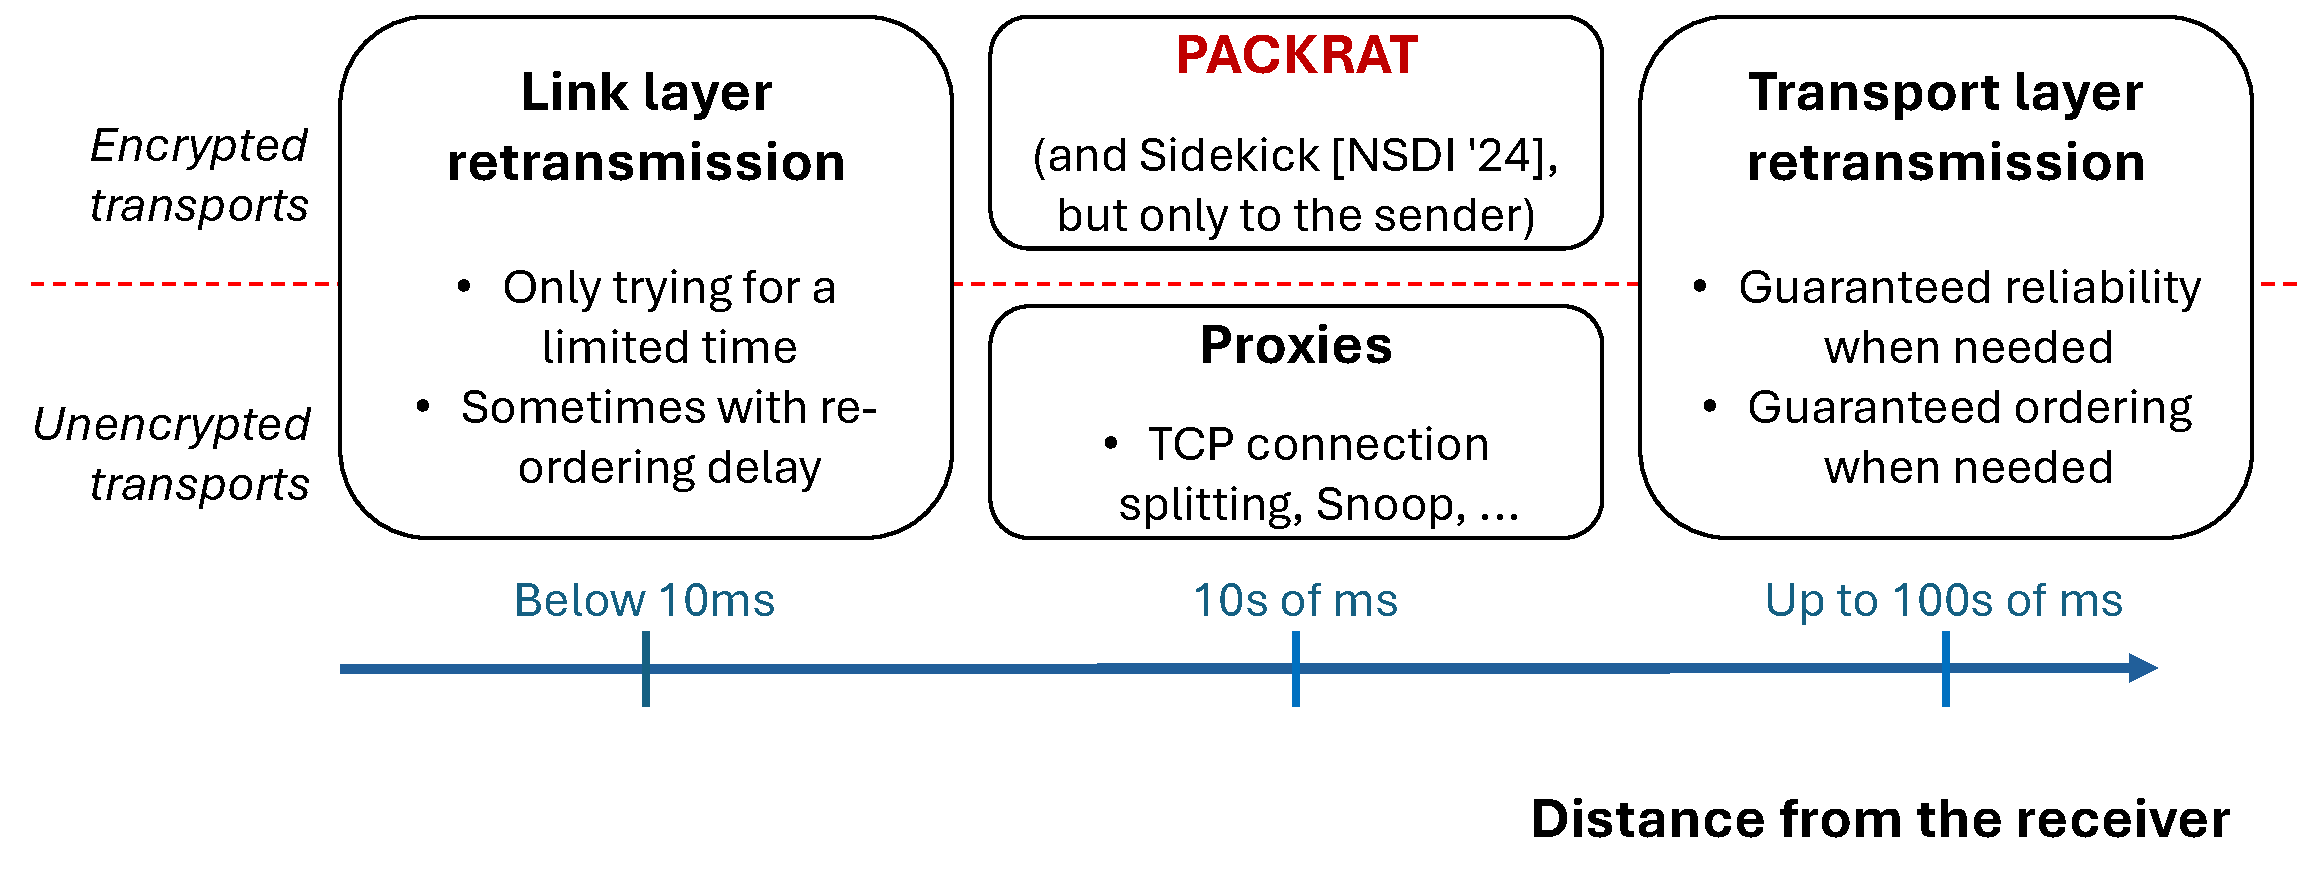
\includegraphics[width=\linewidth,height=35mm]{figures/packrat-scope.pdf}
%     \caption{Just a suggestion from Michael, to include a diagram like this. The editable pptx file is in the figures folder.}
%     \label{fig:packrat-scope}
% \end{figure}

We integrate the \Sys protocol with several applications built on encrypted
transport protocols, and show that it can enable a variety of performance
enhancements in various settings with a lossy path segment near the data receiver,
compared to end-to-end loss recovery schemes:

\begin{enumerate}[noitemsep]
\item Application 1: Improved throughput for large file downloads using QUIC and HTTP/3.
\item Application 2: Reduced packet tail latency of a low-latency media stream using a simple repetition code.
\item Application 3: Reduced end-to-end retransmissions at the server of a reliable multicast RTP stream.
\end{enumerate}

\noindent Unlike link-layer retransmissions, the assistance from a \Sys can be
deployed anywhere along the network path and tailored to the performance
demands of each base connection. Compared to existing transport-layer
solutions, \Sys can be applied to arbitrary transport protocols without
ossification.

\paragraph{Summary of results.}
To summarize, we show that it is possible to provide per-connection in-network
retransmissions to encrypted transport protocols using the \Sys protocol along
an adjacent connection, without involving the data sender nor modifying the
wire format of the underlying connection. We make the following contributions:

\begin{itemize}[noitemsep]
    \item The \Sys protocol and a mechanism at the \textit{endpoint} to correct
     end-to-end reordering signals when there are in-network retransmissions
     (\Cref{sec:packrat-protocol}).
    \item An acknowledgment of encrypted packets based on the Rateless IBLT
     that is fast to decode (\Cref{sec:eack}).
    \item Optimizations to improve proxy
     scalability based on the co-location of the endpoint and eACK sender
     (\Cref{sec:eack:hints}).
    \item An implementation of the \Sys proxy and integrations with three
     applications that use encrypted transport (\Cref{sec:implementation}).
    \item An emulation study of the performance enhancements, as well as the CPU,
     memory, and link overheads of using the \Sys protocol (\Cref{sec:evaluation}).
    % \item Real-world experiments using an in-line commodity device behind a Wi-Fi AP as the \Sys.
\end{itemize}
